\documentclass[12pt]{article}

\usepackage[margin=1 in]{geometry}

%Use Times New Roman font
%\usepackage{pslatex}

% allow text colors
\usepackage[usenames,dvipsnames,svgnames,table,x11names]{xcolor}

%allow double-spacing
\usepackage{setspace}

%enable support for figures
\usepackage{graphicx}

\usepackage{rotating}
\usepackage{multirow}

\usepackage{url}

%handle filenames better
\usepackage{grffile}

%math
%\usepackage{mathtools}
\usepackage{amsmath}
\usepackage{amsfonts}
\usepackage{lipsum}

%control figure movement
\usepackage{placeins}

%center captions
\usepackage{caption}

%circuits and units
\usepackage[free-standing-units]{siunitx}
\DeclareSIUnit\vrms{\volt{}_{RMS}}
%\usepackage[americanvoltages,americancurrents]{circuitikz}
%\usetikzlibrary{calc}

% make scientific notation easy
\providecommand{\e}[1]{\ensuremath{\times 10^{#1}}}

% include pdf documents
\usepackage{pdfpages}

%for loops
\usepackage{pgffor}

%indent after new sections
\usepackage{indentfirst}

\usepackage{verbatim}

% allow greek letters outside math mode. \text<name of letter>
%\usepackage{textgreek}

% margin editing
\usepackage{changepage}

% braket notation, other goodies
\usepackage{physics}
\usepackage{braket}

%source code
\usepackage{listings}

%hyperlink support
\usepackage{hyperref}

% bibtex support
\usepackage{natbib}

%settings for Python code
%\lstset{basicstyle=\footnotesize\ttfamily,
%commentstyle=\color{OliveGreen},
%keywordstyle=\color{blue},
%tabsize=4,
%numbers=left,
%stringstyle=\color{red},
%language=Python,
%inputencoding=utf8,
%extendedchars=true,
%showstringspaces=flase,
% }

\begin{document}
\singlespacing
\title{Final Report\\
AST 383}
\date{Dec 15 2015}
\author{Robert Rosati \\ Maria Jose Bustamante Rosell}
\maketitle

\begin{abstract}
\par Blah blah blah. Clusters are pretty man.
\end{abstract}

\doublespacing

\section{Clustering Algorithms}

\subsection{DBSCAN}

\subsection{FIDEPE}

FIDEPE (FInd DEnsity PEaks) algorithm \cite{FIDEPE} considers two criteria per point: Local Density and Minimum Distance to a point of higher density.

Local density (\textbf{Rho}), is defined as the number of points $j$ in the "neighborbood"; points closer than $d_c$ from point $i$.
\begin{align*}
	\rho_i = \sum_j \chi(d_{ij}-d_c)
\end{align*}
 where 

\section{Plots}

\begin{figure}[ht]
\centering
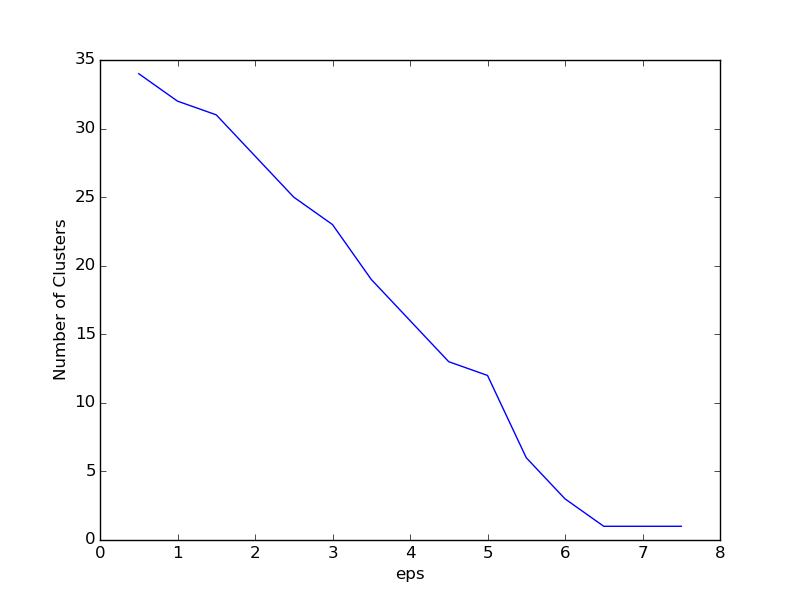
\includegraphics[scale=0.8]{plots/D31_eps}
\caption{The D31 reference distribution.}
\label{fig:panmotor}
\end{figure}


\clearpage
\bibliographystyle{plain}
\bibliography{research}

\end{document}
